\documentclass[a4paper,11.5pt]{article}
\usepackage[textwidth=170mm, textheight=230mm, inner=20mm, top=20mm, bottom=30mm]{geometry}
\usepackage[normalem]{ulem}
\usepackage[utf8]{inputenc}
\usepackage[T1]{fontenc}
\PassOptionsToPackage{defaults=hu-min}{magyar.ldf}
\usepackage{pgfplots}
\pgfplotsset{compat=1.10}
\usepgfplotslibrary{fillbetween}
\usepackage[magyar]{babel}
\usepackage{amsmath, amsthm,amssymb,paralist,array, ellipsis, graphicx, float, bigints,tikz}
%\usepackage{marvosym}

\makeatletter
\renewcommand*{\mathellipsis}{%
	\mathinner{%
		\kern\ellipsisbeforegap%
		{\ldotp}\kern\ellipsisgap
		{\ldotp}\kern\ellipsisgap%
		{\ldotp}\kern\ellipsisaftergap%
	}%
}
\renewcommand*{\dotsb@}{%
	\mathinner{%
		\kern\ellipsisbeforegap%
		{\cdotp}\kern\ellipsisgap%
		{\cdotp}\kern\ellipsisgap%
		{\cdotp}\kern\ellipsisaftergap%
	}%
}
\renewcommand*{\@cdots}{%
	\mathinner{%
		\kern\ellipsisbeforegap%
		{\cdotp}\kern\ellipsisgap%
		{\cdotp}\kern\ellipsisgap%
		{\cdotp}\kern\ellipsisaftergap%
	}%
}
\renewcommand*{\ellipsis@default}{%
	\ellipsis@before
	\kern\ellipsisbeforegap
	.\kern\ellipsisgap
	.\kern\ellipsisgap
	.\kern\ellipsisgap
	\ellipsis@after\relax}
\renewcommand*{\ellipsis@centered}{%
	\ellipsis@before
	\kern\ellipsisbeforegap
	.\kern\ellipsisgap
	.\kern\ellipsisgap
	.\kern\ellipsisaftergap
	\ellipsis@after\relax}
\AtBeginDocument{%
	\DeclareRobustCommand*{\dots}{%
		\ifmmode\@xp\mdots@\else\@xp\textellipsis\fi}}
\def\ellipsisgap{.1em}
\def\ellipsisbeforegap{.05em}
\def\ellipsisaftergap{.05em}
\makeatother

\usepackage{hyperref}
\hypersetup{
	colorlinks = true	
}

\DeclareMathOperator{\Int}{int}
\DeclareMathOperator{\tg}{tg}
\DeclareMathOperator{\ctg}{ctg}
\DeclareMathOperator{\Th}{th}
\DeclareMathOperator{\sh}{sh}
\DeclareMathOperator{\ch}{ch}
\DeclareMathOperator{\arsh}{arsh}
\DeclareMathOperator{\arch}{arch}
\DeclareMathOperator{\arth}{arth}
\DeclareMathOperator{\arcth}{arcth}
\DeclareMathOperator{\arc}{arc}
\DeclareMathOperator{\arctg}{arc tg}
\DeclareMathOperator{\arcctg}{arc ctg}
\newcommand{\norm}[1]{\left\lVert#1\right\rVert}

\begin{document}
	%%%%%%%%%%%RÖVIDÍTÉSEK%%%%%%%%%%
	\setlength\parindent{0pt}
	\def\a{\textbf{a}}
	\def\b{\textbf{b}}
	\def\N{\hskip 10 true mm}
	\def\a{\textbf{a}}
	\def\b{\textbf{b}}
	\def\c{\textbf{c}}
	\def\d{\textbf{d}}
	\def\e{\textbf{e}}
	\def\gg{$\gamma$}
	\def\vi{\textbf{i}}
	\def\jj{\textbf{j}}
	\def\kk{\textbf{k}}
	\def\fh{\overrightarrow}
	\def\l{\lambda}
	\def\m{\mu}
	\def\v{\textbf{v}}
	\def\0{\textbf{0}}
	\def\s{\hspace{0.2mm}\vphantom{\beta}}
	\def\Z{\mathbb{Z}}
	\def\Q{\mathbb{Q}}
	\def\R{\mathbb{R}}
	\def\C{\mathbb{C}}
	\def\N{\mathbb{N}}
	\def\Rn{\mathbb{R}^{n}}
	\def\Ra{\overline{\mathbb{R}}}
	\def\sume{\displaystyle\sum_{n=1}^{+\infty}}
	\def\sumn{\displaystyle\sum_{n=0}^{+\infty}}
	\def\biz{\emph{Bizonyítás:\ }}
	\def\narrow{\underset{n\rightarrow+\infty}{\longrightarrow}}
	\def\limn{\displaystyle\lim_{n\to +\infty}}
	%	\def\definition{\textbf{Definíció:\ }}
	%	\def\theorem{\textbf{Tétel:\ }}
	%\def\note{\emph{Megjegyzés:\ }}
	%\def\example{\textbf{Példa:\ }} 
	
	\theoremstyle{definition}
	\newtheorem{theorem}{Tétel}[subsubsection] % reset theorem numbering for each chapter
	
	\theoremstyle{definition}
	\newtheorem{definition}[theorem]{Definíció} % definition numbers are dependent on theorem numbers
	\newtheorem{example}[theorem]{Példa} % same for example numbers
	\newtheorem{exercise}[theorem]{Házi feladat} % same for example numbers
	\newtheorem{note}[theorem]{Megjegyzés} % same for example numbers
	\newtheorem{task}[theorem]{Feladat} % same for example numbers
	\newtheorem{revision}[theorem]{Emlékeztető} % same for example numbers
	%%%%%%%%%%%%%%%%%%%%%%%%%%%%%%%%%
	\begin{center}
		{\LARGE\textbf{Analízis 3. A szakirány}}
		\smallskip
		
		{\Large Gyakorlati jegyzet}
		
		\smallskip
		7. óra.
	\end{center}
	A jegyzetet \textsc{Umann} Kristóf készítette \textsc{Filipp} Zoltán István gyakorlatán. (\today)
	\section{Többáváltozós függvények analízise}
	\subsection{Személtetés $\R^2\to\R$ esetre}
	\begin{note}
		Példa lehet alkalmazására pl. egy sík terület adott pontjához annak hőmérsékletének hozzárendelése.
	\end{note}
	\begin{note}
		Világos, hogy a $\R^2\to\R$ függvények ábrázolásához szükséges lesz egy új, $z$ tengelyre.
	\end{note}
	\begin{task}
		\[ f(x,y):=x^2+y^2\quad ((x,y)\in\R^2)\quad \Leftrightarrow\quad z=y^2+y^2 \]
		Az ilyen függvényeket úgy fogjuk tudni megoldani, hogy a függvény képéből kimetszünk egy görbét, melynek segítségével már vizsgálható az az adott rész egyváltozós analízissel.
		
		\medskip
		Megállapítható, hogy $\forall (x,y)\in\R^2:\quad z>0$.
		\smallskip
		Szintvonalak: (vagy vízszintes metszetek)
		\begin{align*}
			z=0&\quad \Leftrightarrow\quad x^2+y^2=0\quad \Leftrightarrow\quad (x,y)=(0,0) \\
			z=1&\quad \Leftrightarrow\quad x^2+y^2=1\quad \Leftrightarrow\quad \text{1 sugarú körvonal} \\
			z=2&\quad \Leftrightarrow\quad x^2+y^2=(\sqrt{2})^2\quad \Leftrightarrow\quad \text{$\sqrt{2}$ sugarú körvonal} \\
			0<z&\quad \Leftrightarrow\quad x^2+y^2=(\sqrt{z})^2\quad \Leftrightarrow\quad \sqrt{z}\text{ sugarú körvonal} 
		\end{align*}
		\begin{figure}[H]
			\centering
			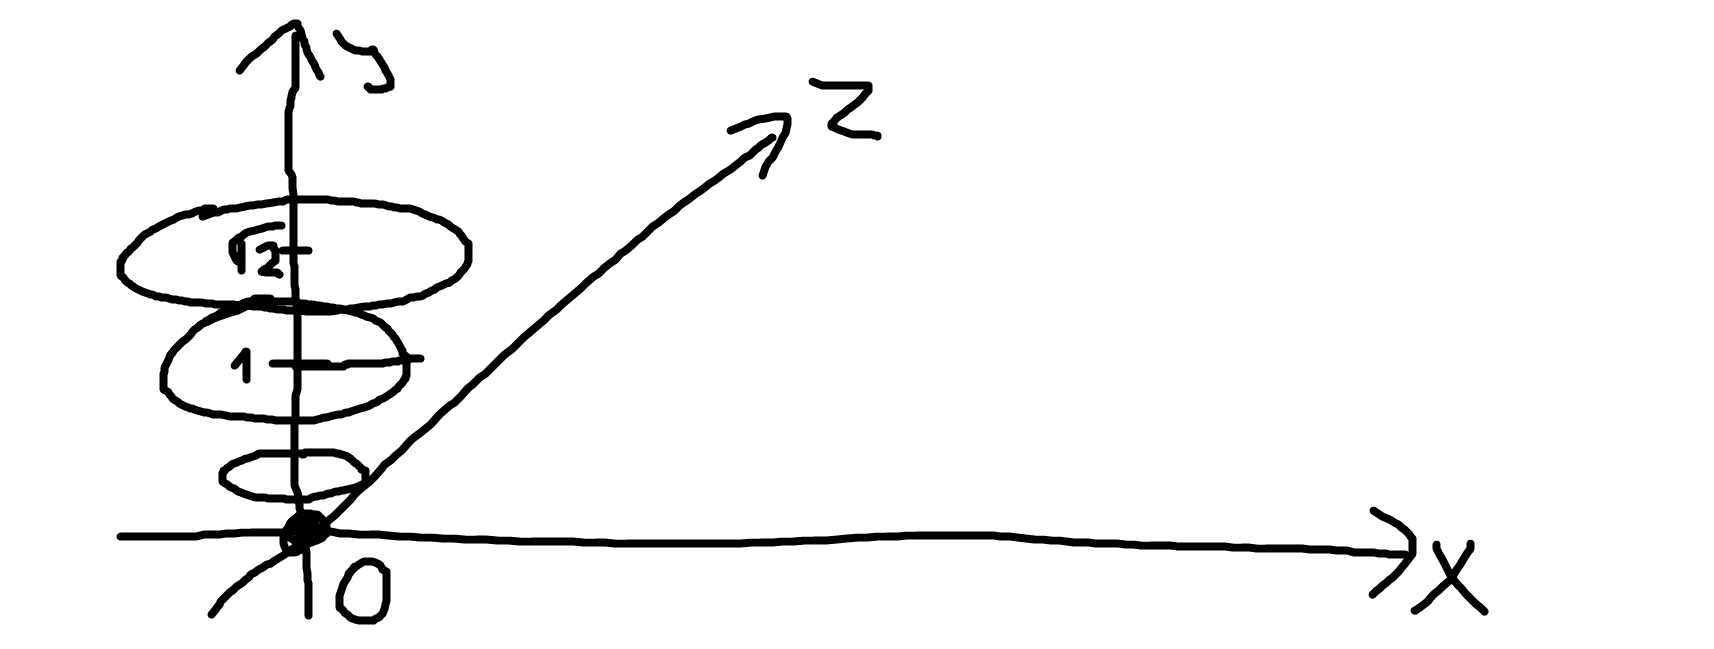
\includegraphics[height=3cm]{kepek/01.png}
			\caption{}
		\end{figure}
		Függőleges metszetek (bizonyos irányok mentén)
		\begin{align*}
			y=0&\quad \Leftrightarrow\quad \text{,,$x$ tengely''}\quad \Rightarrow\quad z=x^2=f(x,0)\quad (x\in\R) \\
			x=0&\quad \Leftrightarrow\quad \text{,,$y$ tengely''}\quad \Rightarrow\quad z=y^2=f(0,y)\quad (x\in\R) \\
			y=x&\quad \text{mentén}\quad \Rightarrow\quad x=f(x,x)=2x^2\quad (y\in\R) 
		\end{align*}
		Ezt a felületet \textit{forgás-paraboloid}nak hívjuk.
		\begin{figure}[H]
			\centering
			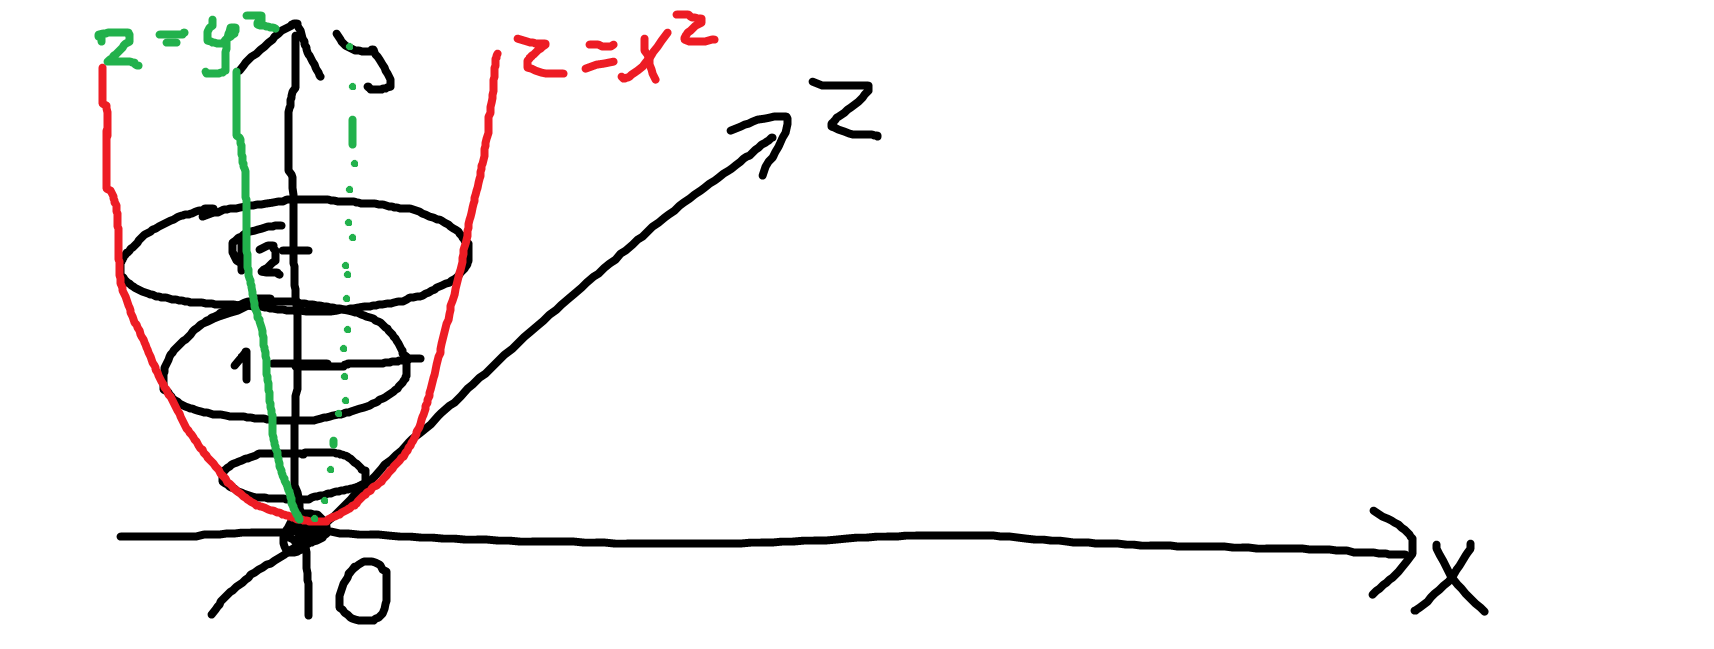
\includegraphics[height=3cm]{kepek/02.png}
			\caption{}
		\end{figure}
	\end{task}
	\begin{note}
		Megállapítható, hogy illeszthető $z=0$-ban érintősík.
	\end{note}
	\begin{task}
		\[ z:=f(x,y):=(\sqrt{x^2+y^2})\quad ((x,y)\in\R^2, z\geq 0) \]
		Szintvonalak:
		\[ z=0\quad \Leftrightarrow\quad \sqrt{x^2+y^2}=0\quad \Leftrightarrow\quad (x,y)=(0,0) \]
		\[ z=1\quad \Leftrightarrow\quad \sqrt{x^2+y^2}=1\quad \Leftrightarrow\quad x^2+y^2=1^2 \]
		\[ z=2\quad \Leftrightarrow\quad \sqrt{x^2+y^2}=2\quad \Leftrightarrow\quad x^2+y^2=2^2 \]
		\begin{figure}[H]
			\centering
			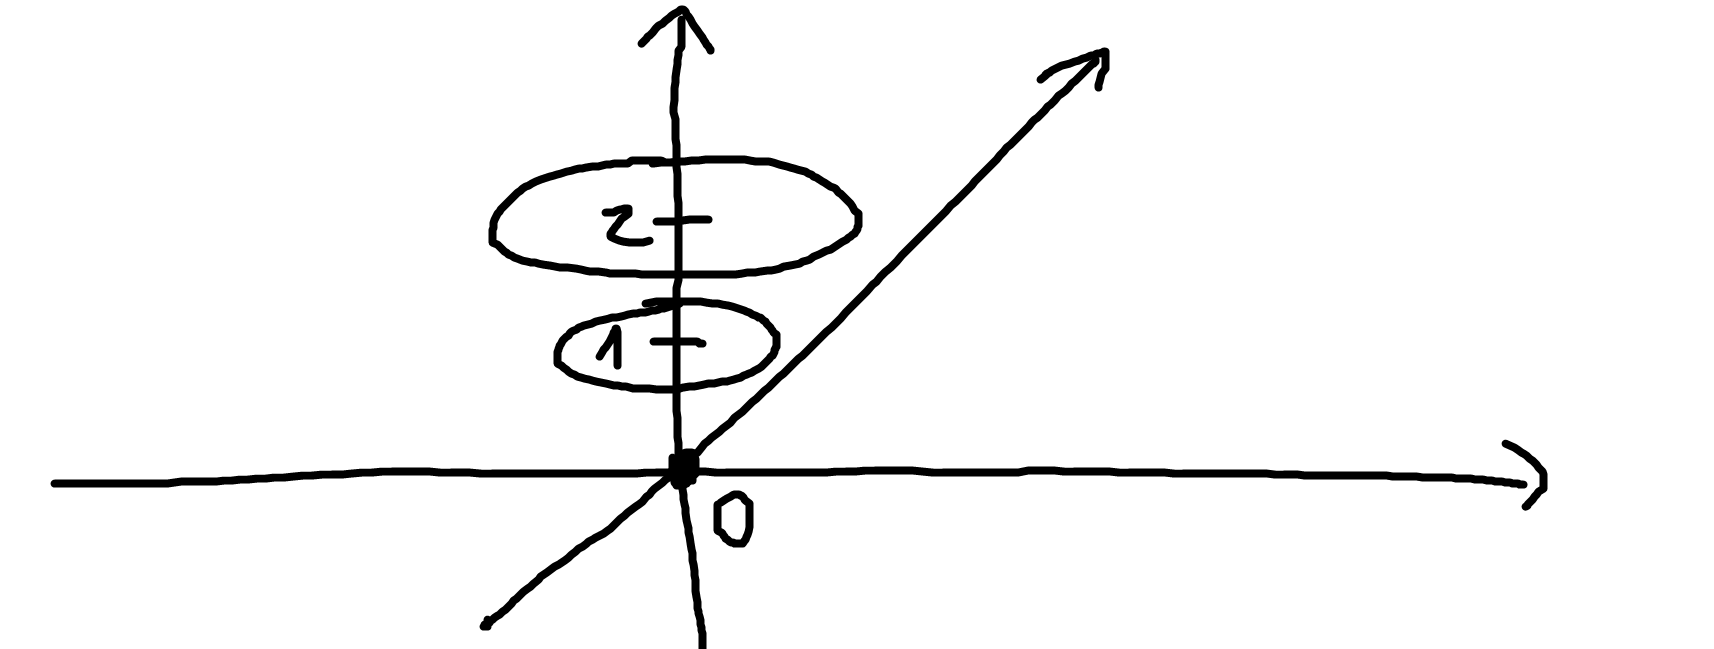
\includegraphics[height=3cm]{kepek/03.png}
			\caption{}
		\end{figure}
		Függőleges metszetek:
		\[ y=0\quad \Rightarrow\quad z=\sqrt{x^2}=|x|=f(x,0)\quad (x\in\R) \]
		\[ x=0\quad \Rightarrow\quad z=\sqrt{y^2}=|y|=f(0,y)\quad (y\in\R) \]
		Ez a már jól ismert \textit{kúp}.
		\begin{figure}[H]
			\centering
			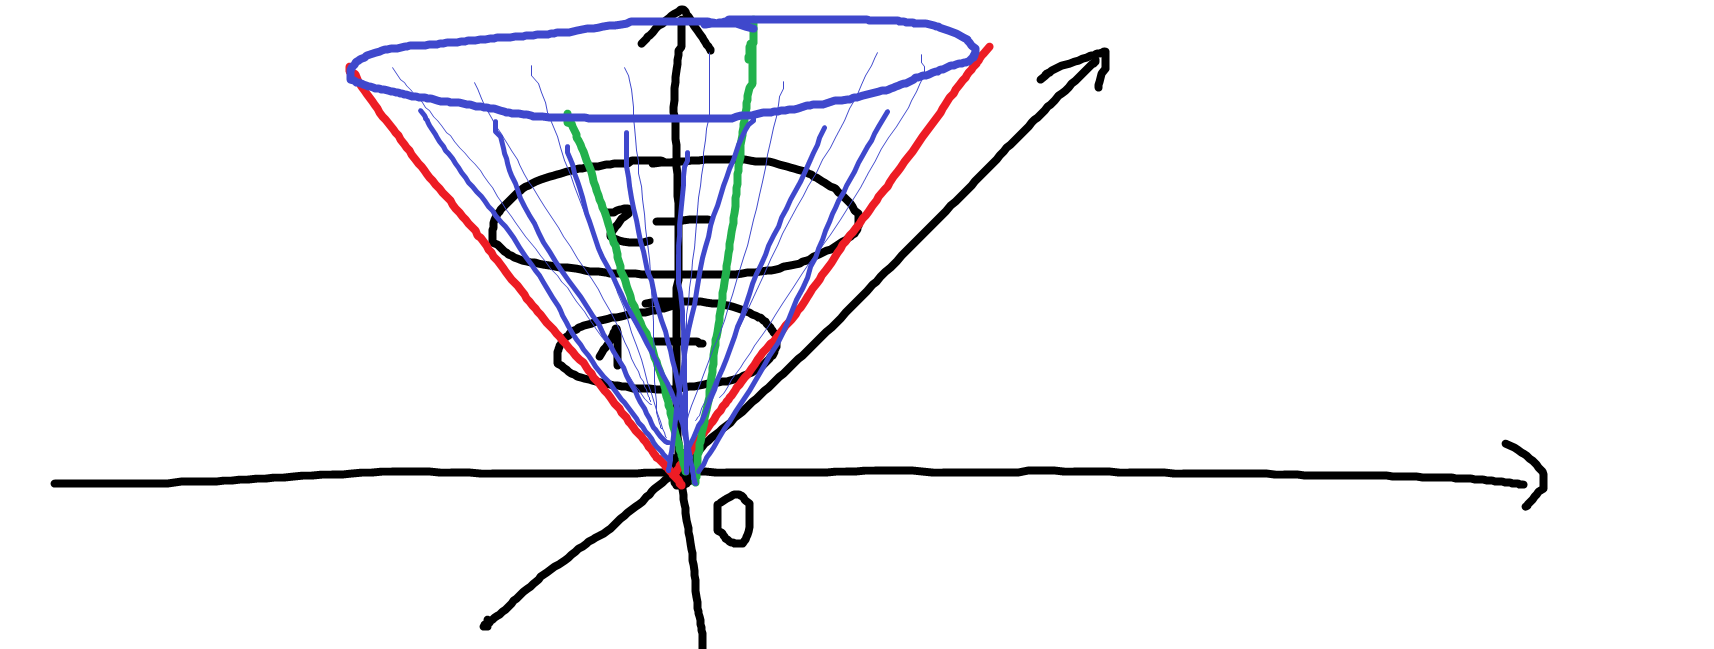
\includegraphics[height=3cm]{kepek/04.png}
			\caption{}
		\end{figure}
	\end{task}
	\begin{note}
		Megálapítható, hogy $z=0$-ra nem tudunk érintősíkot illeszteni.
	\end{note}
	\begin{task}Keresük a legbővebb halmazt, ahol ez függvényként értelmezhető
		\[ f(x,y):=\sqrt{1-x^2-y^2}=z,\quad ((x,y)\in\mathcal{D}_f=?) \]
		Világos, mikor értelmezhető.
		\[ \mathcal{D}_f=\left\{(x,y)\in\R^2~|~\sqrt{x^2+y^2}\leq 1 \right\}=\left\{ (x,y)\in\R^2~|~\norm{(x,y)-(0,0)}_2\leq 1 \right\} \]
		Ezek azok a pontok, melyek az origótól 1 távolságra vannak.
		\begin{figure}[H]
			\centering
			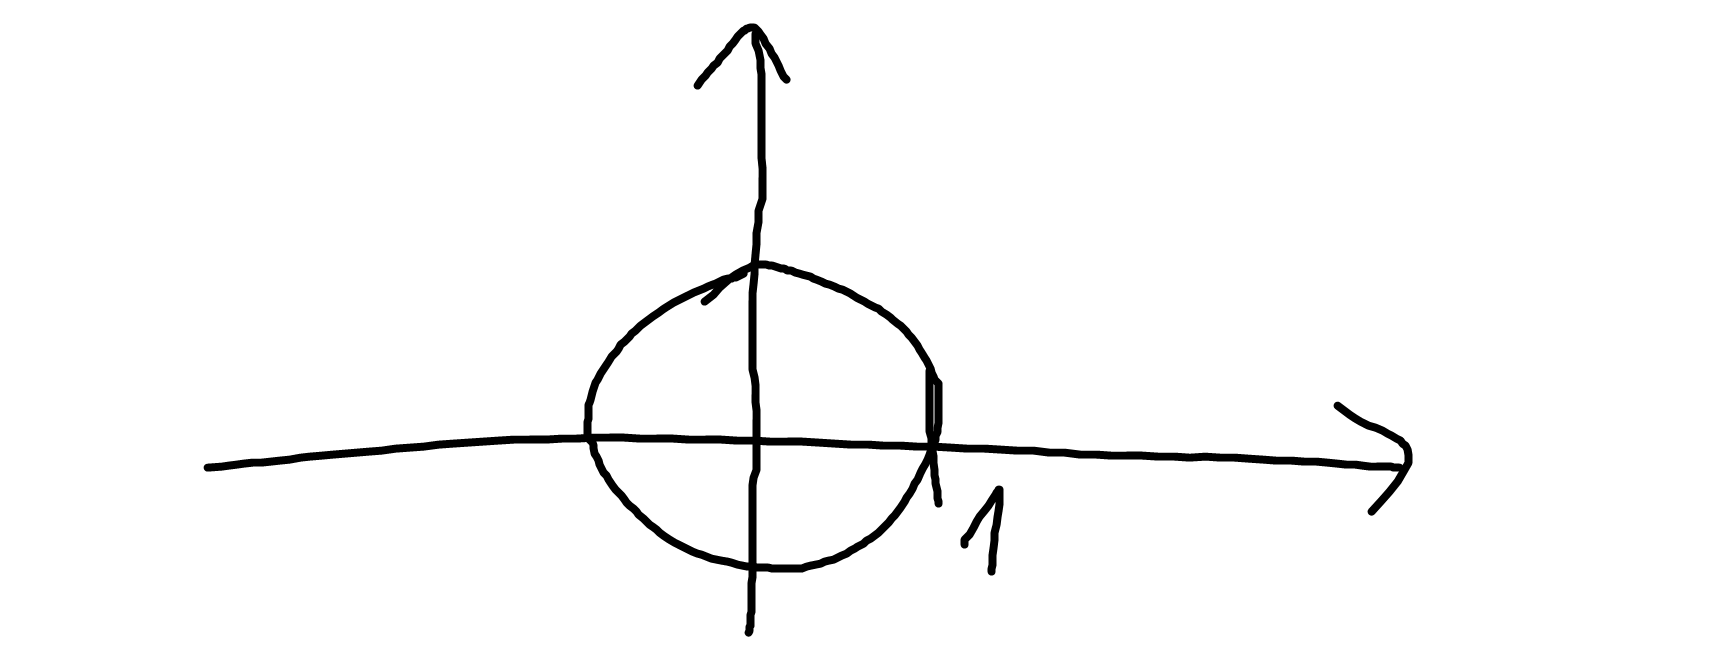
\includegraphics[height=3cm]{kepek/05.png}
			\caption{}
		\end{figure}
		Megállapítható, hogy 1 és $-1$-en kívül nincsenek függvényértékek.
		\smallskip
		
		Síkvonalak:
		\begin{align*}
			x=0&\quad \Rightarrow\quad \sqrt{1-x^2-y^2}=0\quad \Leftrightarrow\quad x^2+y^2=1 \quad \text{(ábrán fekete körvonal)}\\
			x=1&\quad \Rightarrow\quad \sqrt{1-x^2-y^2}=1\quad \Leftrightarrow\quad x^2+y^2=0\quad \Rightarrow\quad (x,y)=(0,0) \\
			x=\frac{1}{2}&\quad \Rightarrow\quad \sqrt{1-x^2-y^2}=\frac{1}{2}\quad \Leftrightarrow\quad x^2+y^2=\frac{3}{4}=\left(\frac{a\sqrt{3}}{2}\right)^2 \quad \text{(ábrán zöld körvonal)}
		\end{align*}
		Függőleges
		\[ x=0\quad \text{mentén}\quad \Rightarrow\quad z=f(x,0)=\sqrt{1-x^2}\quad x\in[-1,1]\quad \text{ábrán piros félkörvonal} \]
		\[ y=0\quad \text{mentén}\quad \Rightarrow\quad  z=f(0,y)=\sqrt{1-y^2}\quad y\in[-1,1]\quad \text{ábrán kék félkörvonal} \]
		\begin{figure}[H]
			\centering
			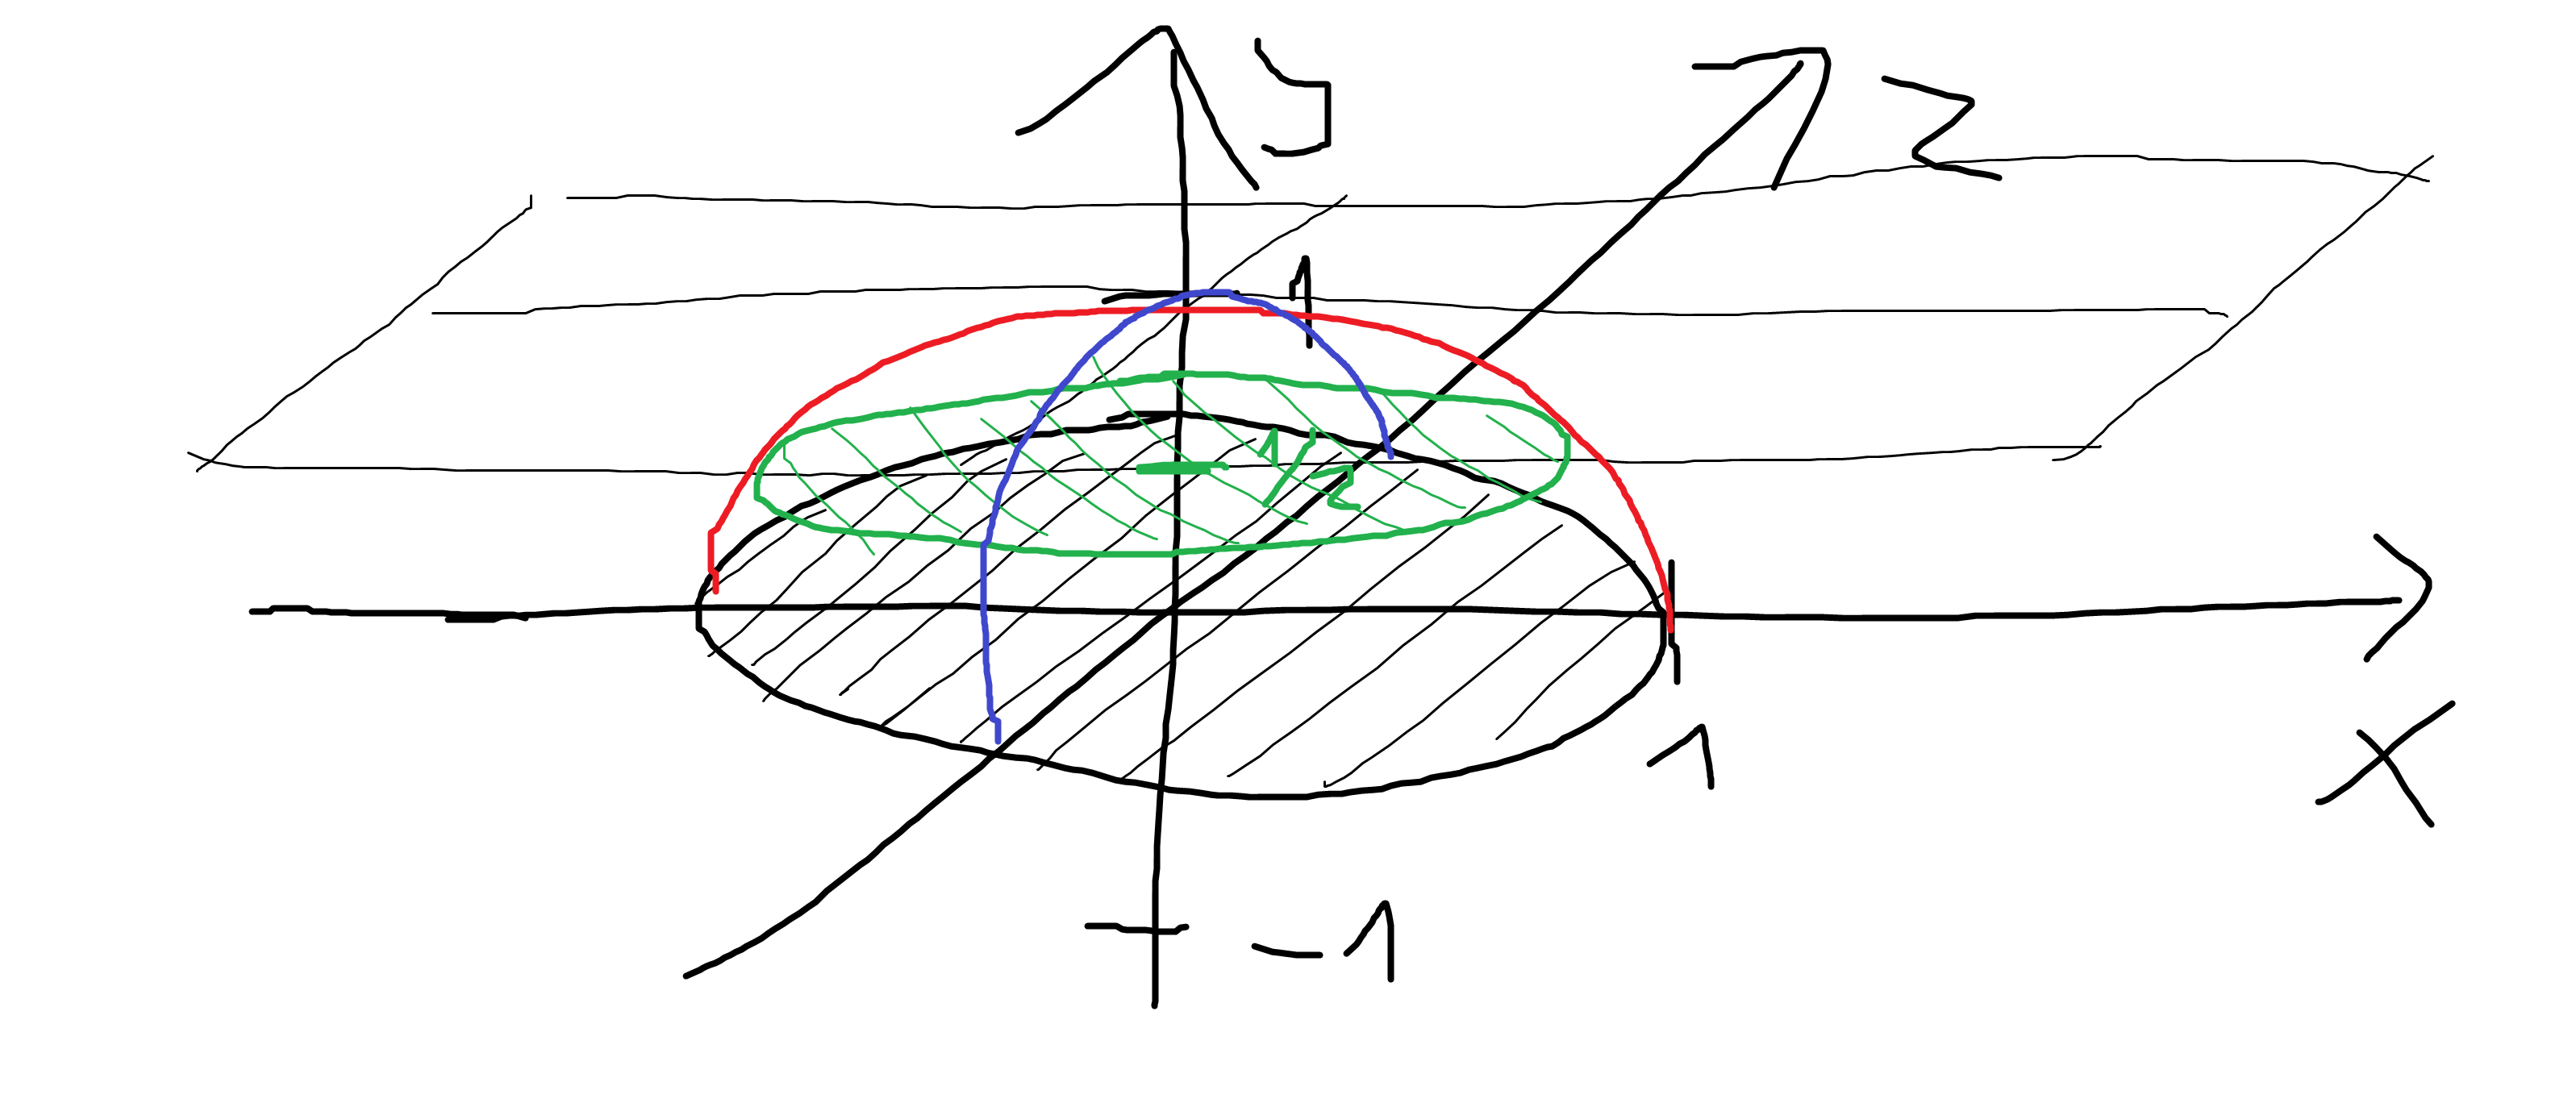
\includegraphics[height=3cm]{kepek/06.png}
			\caption{}
		\end{figure}
	\end{task}
	\begin{exercise}
		\[ z:=f(x,y):=e^{-x^2-y^2}\quad (x,y)\in\R^2 \]
		Szemléltessük!
	\end{exercise}
	\begin{note}
		Irodalom:
		\begin{enumerate}
			\item Gyemidovics
			\item Bolyai sorozat (többváltozós függvények analízise)
			\item Szili László
			\item Kórolyi Katalin $\rightarrow$ honlap
		\end{enumerate}
	\end{note}
	\subsection{Határérték számítása}
	\begin{revision} (határérték definíciója és átviteli elv)
		\begin{enumerate}
			\item $f\in\R^n\to\R^m;\quad 1\leq n,m\in\N;\quad a\in\mathcal{D}_f',\quad A\in\R^m$:
			\[ \lim_{x\to a}f(x)=\lim_af=A\quad \overset{\text{def.}}{\Longleftrightarrow}\quad \forall\varepsilon>0\quad \exists\partial>0\quad \forall x\in\mathcal{D}_f\setminus\{a\}:\quad 0<||x-a||_{\R^n}<\partial\quad ||f(x)-A||_{\R^m}<\varepsilon \]
			\item (átviteli elv)\[ \forall (x_k):\N\to\R^n\setminus\{a\}\quad \text{és}\quad \lim_{k\to\infty}(x_k)=a:\quad \lim_{k\to\infty}f(x_k)=A \]
		\end{enumerate}
	\end{revision}
	\begin{task} $(x,y)\in\R^2,\quad x^2+y^2\not=0$
		\[ \lim_{(x,y)\to\underbrace{(1,2)}_{a}}\left(\frac{x^2+xy}{x+y^2}\right)=\frac{1^2+1\cdot2}{1+2^2}=\frac{3}{5} \]
	\end{task}
	Miért tehetjük meg azt, hogy itt többváltoznál is simán beírhatjuk az értékeket?
	\begin{task}
		\[ \lim_{(x,y)\to(6,3)}x\cdot y\cdot\cos(x-2y)=18\cdot\cos0=18 \]
		Ugyanis: ld. átviteli elv. Tekintsünk egy vektorsorozatot, melyre
		\[ \underbrace{(x,y)}_{\not=(6,3)}\to(6,3)\quad (n\to\infty)\quad \Leftrightarrow\quad  \]
		Ez akkor és csak akkor konvergens, ha komponensenként konvergál.
		\[\begin{cases}
			\lim(x_n)=6\\
			\lim(y_n)=3
		\end{cases} \Rightarrow\quad \exists\lim(x_n,y_n)\quad \text{és}\quad \lim(x_n,y_n)=6\cdot3\cdot1=18 \]
		Válasszunk meg egy valós sorozatot. Szerencsés, ha ez 0-hoz tart. %TODO sure?
		\[ u_n:=x_n-2y_n\to 6-2\cdot3=0\quad (n\to\infty) \]
		Legyen 
		\[ g(t):=\cos t\quad (t\in\R)\quad (g\in\R\to\R) \]
		Hatványsorozatok összege folytonos, így alkalmazható az átviteli elv
		\[ g\in C\quad \Rightarrow\quad \exists\lim_{n\to\infty}\cos(x_n-2y_n)\quad \text{és}\quad \lim_{n\to\infty}\cos(x_n-2y_n)=1 \]
		Ahol kihasználtuk, hogy $u_n\to0\quad \Rightarrow\quad \cos(u_n)\to\cos 0=1\quad (n\to\infty)$
	\end{task}
	\begin{task}
		\[ \lim_{(x,y)\to(0,0)}\frac{x^2+y^2}{\sqrt{x^2+y^2+1}-1}\quad \overset{\frac{0}{0}}{=}\quad \lim_{(x,y)\to(0,0)}\frac{(x^2+y^2)(\sqrt{x^2+y^2+1}+1)}{x^2+y^2+1-1}=\sqrt{1}+1=2 \]
	\end{task}
	\begin{task}$(x,y)\in\R^2\setminus\{(0,0)\}$
		\[ \lim_{(x,y)\to(0,0)}\overbrace{\frac{x^2}{x^2+y^2}}^{:=f(x,y)}\quad \overset{\frac{0}{0}}{=}\quad  \]
		Sajnos itt nem tudunk tovább haladni hagyományos módszerekkel. Így új módszert kell használnunk.
		\smallskip
		
		Legyen \[\left(\frac{1}{n},0\right)\to(0,0)\quad \text{ha}\quad (n\to\infty)\quad \Rightarrow\quad f\left(\frac{1}{n},0\right)=\frac{\frac{1}{n^2}}{\frac{1}{n^2}+0^2}=1\quad \to1(n\to\infty)\]
		
		$\quad \overset{\text{átv. elv}}{\Rightarrow}$\quad Ha $\exists\lim_{(0,0)}f=1$ \textbf{lehet} csak.
		Legyen 
		\[ \left(0,\frac{1}{n}\right)\to(0,0)\quad \text{ha}\quad (n\to\infty) \]
		\[ \Rightarrow\quad f\left(0,\frac{1}{n}\right)=\frac{0}{\frac{1}{n^2}+0^2}=0\to 0(n\to\infty) \]
		\[ \Rightarrow \text{ha}\quad \exists\lim_{(0,0)}f\quad \text{csak}\quad 0 \quad \text{lehet} \]
		Mivel két kül. határérték nem lehet, nem létezik ez a határérték.
	\end{task}
	\begin{note}
		A cél egy 0-hoz tartó sorozat megválasztása és vizsgálása.
	\end{note}
	\begin{task}
		\[ \lim_{(x,y)\to(0,0)}\frac{x^2y^2}{x^2y^2+(x-y)^2}\quad \overset{\frac{0}{0}}{=}\quad  \]
		Legyen újra
		\[ \left(\frac{1}{n},0\right)=\frac{0}{\left(\frac{1}{n}\right)^2}=0\to0 \]
		Azaz a határérték csak 0 lehet, más nem, ha létezik.
		\[ \left(0,\frac{1}{n}\right)\to(0,0)\quad (n\to\infty)\quad \text{és}\quad  f\left(0,\frac{1}{n}\right)=\frac{0}{\left(\frac{1}{n}\right)^2}=0\to 0\quad (n\to\infty) \]
		De:
%		\[ \left(\frac{1}{n},\frac{1}{n}\right) \to(0,0) (n\to\infty)\quad \text{és}\quad f\left(\frac{1}{n},\frac{1}{n}\right)=\frac{\left(\frac{1}{n}\right)^n}{left(\frac{1}{n}\right)^n+\left(\frac{1}{n}-\frac{1}{n}\right)^2}=1 \]
	\end{task}
	\begin{note}
		Mindig más irányból közelítjük az origót. Rendre $x, y$ és $z$ tengely mentén.
	\end{note}
	\begin{task}
		Bizonyítsuk be, hogy
		\begin{enumerate}
			\item \[ \exists\lim_{x\to0}\left(\lim_{y\to0}\frac{x^2y^2}{x^2y^2+(x-y^2)}\right)=\lim_{x\to0}\left(\frac{1}{x^2}\right)=\lim_{x\to0}(0)=0 \]
			\item \[ \exists\lim_{y\to0}\left(\lim_{x\to0}\frac{x^2y^2}{x^2y^2+(x-y^2)}\right)= \]
			\begin{figure}[H]
				\centering
				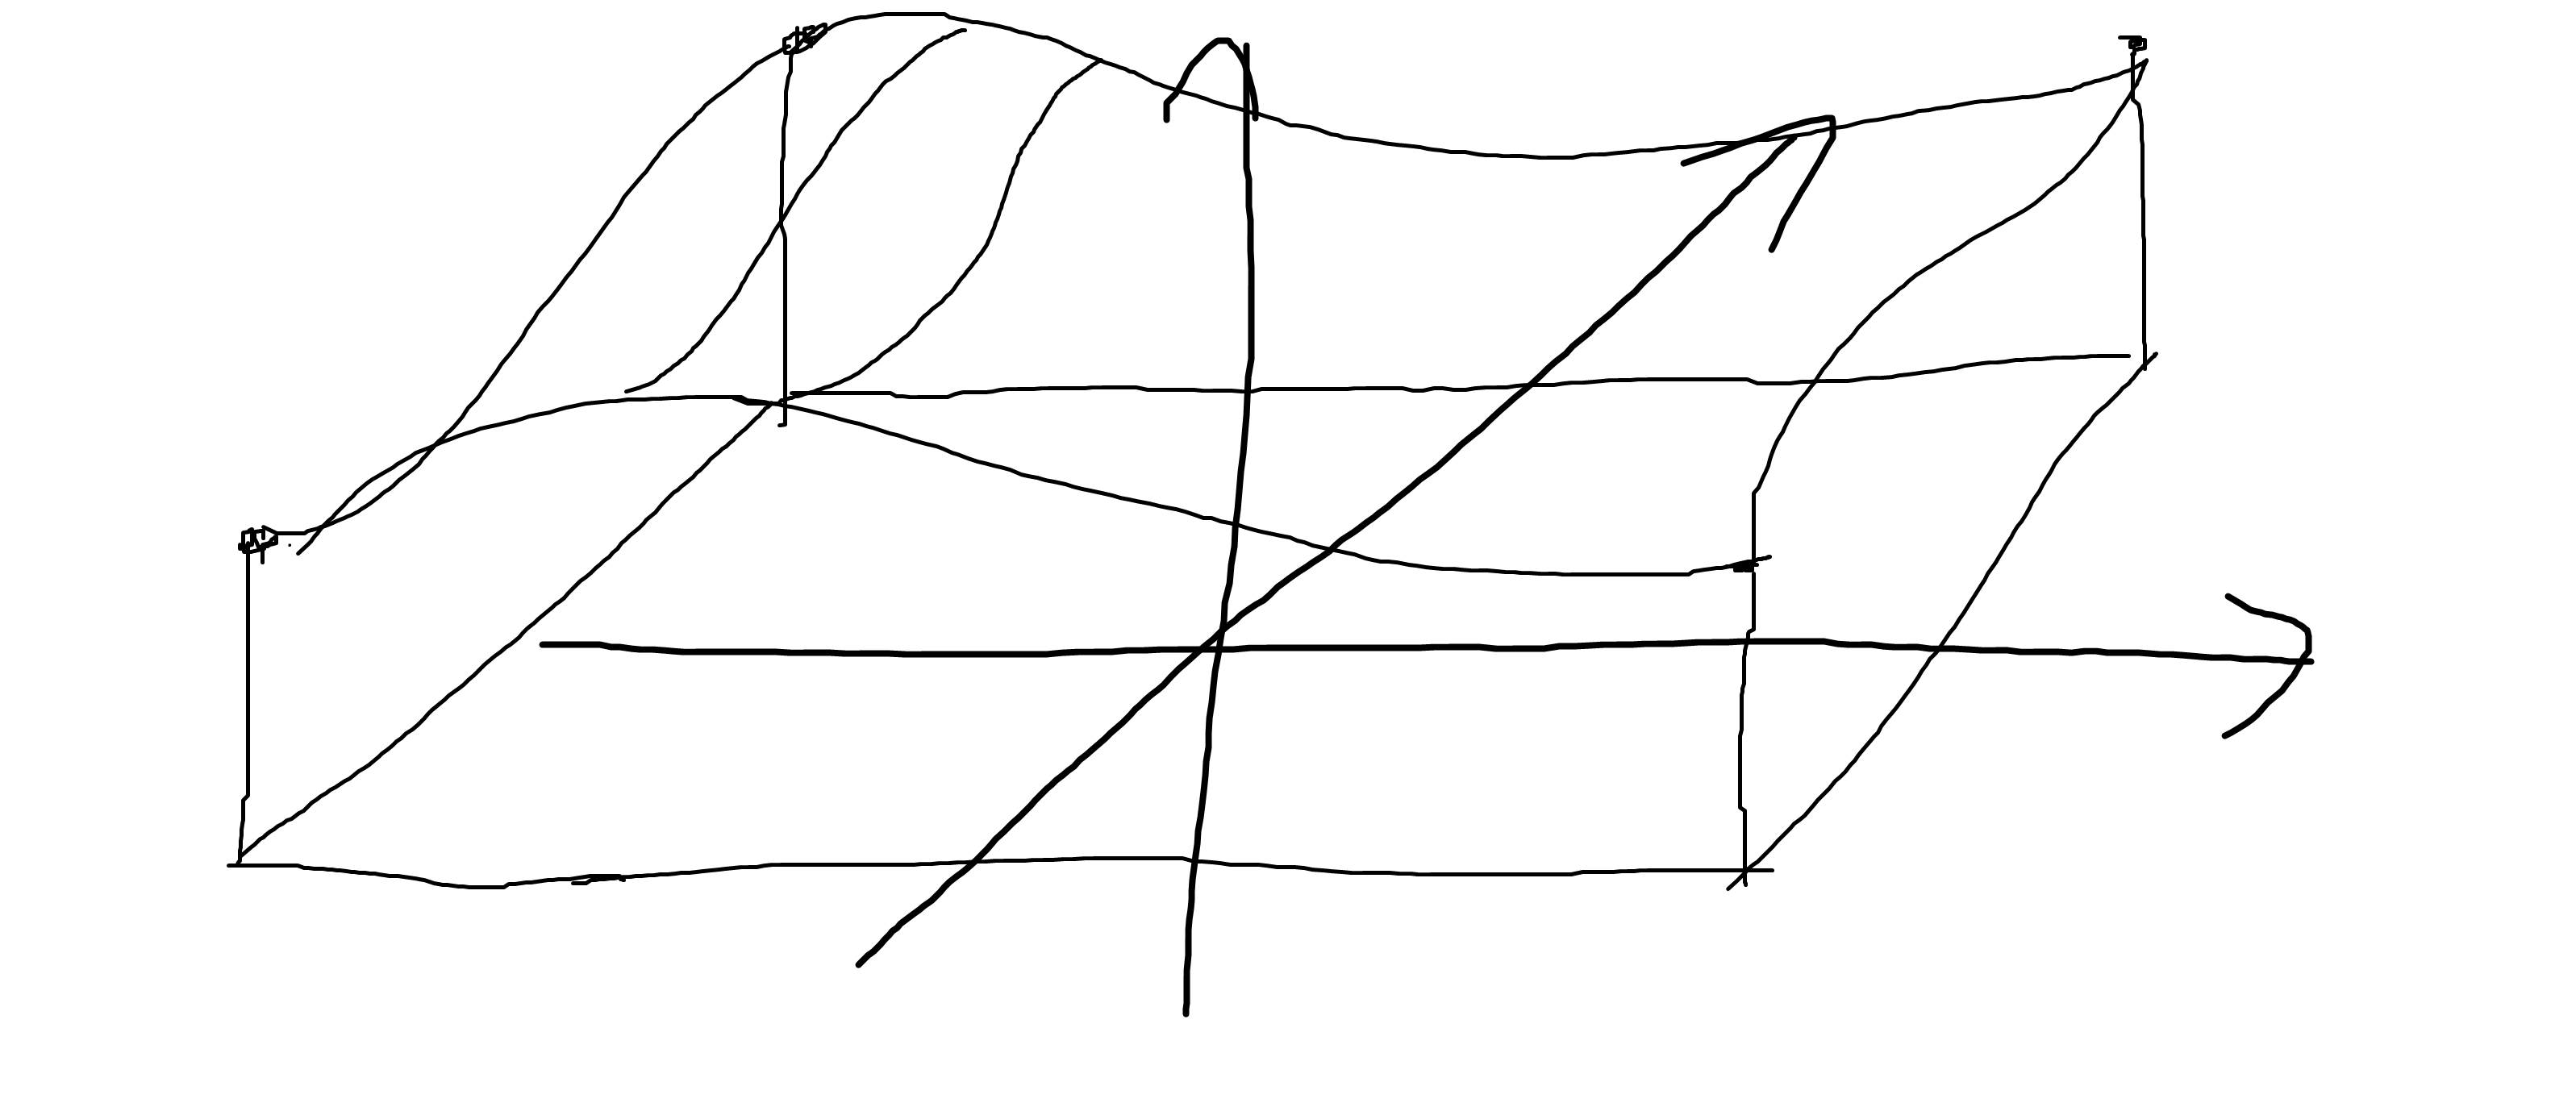
\includegraphics[height=3cm]{kepek/07.png}
				\caption{}
			\end{figure}
			%TODO hiányos 07
		\end{enumerate}
	\end{task}
	\begin{task}
		\[ \lim_{(x,y)\to(0,0)}\left(\frac{xy}{\sqrt{x^2+y^2}}\right) \]
		Rövid jelölés: Sorozatok helyett irányokkal dolgozunk.
		\[ y=0\quad \text{mentén}\quad \Rightarrow\quad \underbrace{f(x,y)}_{x\not=0}=\frac{x\cdot0}{\sqrt{x^2}}=\frac{0}{|x|}=0\to0\quad (\text{ha}\quad x\to0) \]
		Ha $\exists\lim_{(0,0)}f=0$ lehet csak.
		\[ x=0\quad \text{mentén}\quad \Rightarrow\quad f(0,y)=\frac{0\cdot y}{\sqrt{y^2}}=\frac{0}{|y|}=0\to 0 \]
		ha $y\to0$.
		
		\smallskip
		vagy:
		\[ y=x\quad \text{mentén}\quad \Rightarrow\quad g(x):=f(x,x)=\frac{x^2}{\sqrt{2x^2}}=\frac{x^2}{\sqrt{2}\cdot|x|}=\frac{|x|^2}{\sqrt{2}\cdot|x|}=\frac{|x|}{\sqrt{2}}\to0 \]
		Sejtés: $\lim_{(0,0)}f=0$. (lévén nem tudtuk cáfolni)
		
		Definíció alapján:
		\[ \forall\varepsilon>0\quad \exists\partial>0\quad \forall(x,y)\in\mathcal{D}_f=\R^2\setminus\{(0,0)\}:\quad 0<||(x,y)-(0,0)||_{\R^2}<\partial\quad |f(x,y)-0|<\varepsilon \]
		Legyen $\varepsilon>0$ fix; és $|f(x,y)-0|=\left|\frac{xy}{\sqrt{x^2+y^2}}\right|=\frac{|xy|}{\sqrt{x^2+y^2}}$
		
		Mi a cél? $||f(x,y)-0||\leq K||(x,y)-(0,0)||_{\R{^2}}$
		\[ \underset{|xy|=\sqrt{x^2y^2}\leq\frac{x^2+y^2}{2}}{\leq}\quad\frac{x^2+y^2}{2\sqrt{x^2+y^2}}=\frac{1}{2}\sqrt{x^2+y^2}=\frac{1}{2}||(x,y)-(0,0)||_2<\varepsilon  \]
		\[ \Leftrightarrow||(x,y)-(0,0)||_2<2\varepsilon \]
		Legyen $\partial:=2\varepsilon$ jó.
	\end{task}
\end{document}